% begin module continuity-ex2
\begin{frame}
\begin{example} %[Example 2a, p. 114]
Where is this function defined?
\begin{columns}[c]
\column{.4\textwidth}
\[
f(x) = \frac{x^2 - x - 2}{\alert<handout:0 |3>{x - 2}}
\]
\ \uncover<4->{
\psset{xunit=0.8cm, yunit=0.8cm}
\begin{pspicture}(-3, -2)(3,4)
 \psframe*[linecolor=white](-3,-2)(3,4) \psaxes[labels=none]{<->}(0,0)(-3,-2)(3,4)
 \psplot[linecolor=red, plotpoints=1000]{-3}{3}{x 1 add }
 \fcHollowDot{2}{3}
\end{pspicture} %
%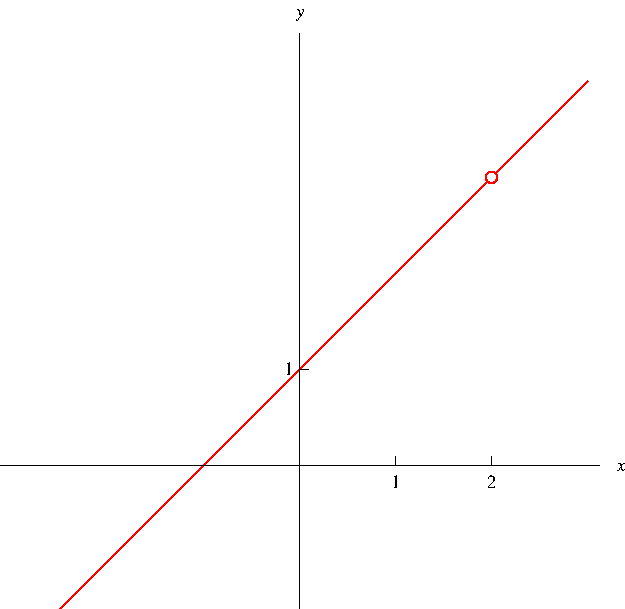
\includegraphics[height=4.5cm]{continuity/pictures/02-05-ex2a.pdf}%
}
\column{.6\textwidth}
\begin{itemize} \frametitle{Removable Discontinuity}
\item<2-| alert@2-3>  $f(2)$ \uncover<3->{is not defined.}
%\item<4->  Discontinuous at 2. %Todor: I disagree: the function is not defined at 2, rather than discontinuous.
\item<4->  This is called a removable discontinuity because we could redefine the value of $f$ at a single number $x = 2$ to make $f$  continuous at that point.
\end{itemize}
\begin{definition}<5->
In general, $ f $ has a \textbf{removable discontinuity} at $ x=a $ if $ \ds \lim_{x\to a}f(x) $ exists, but is not equal to $ f(a). $
\end{definition}
\end{columns}
\end{example}
\end{frame}


\begin{frame} \frametitle{Infinite Discontinuity}
\begin{example} %[Example 2b, p. 114]
Where is this function discontinuous?
\begin{columns}[c]
\column{.4\textwidth}
\[
f(x) = \left\{ \begin{array}{lcl}
\frac{1}{\alert<handout:0 |6>{x^2}} & \text{ if } & x \neq 0 \\
\alert<handout:0 |4>{1} & \alert<handout:0 |4>{\text{ if }} & \alert<handout:0 |4>{x = 0} \\
\end{array}\right.
\]
\psset{xunit=0.8cm, yunit=0.8cm}
\begin{pspicture}(-3.1, -0.5)(5.1,3.1) \psframe*[linecolor=white](-3.1,-0.5)(3,5)
\psaxes[ticks=x, labels=none]{<->}(0,0)(-3,-0.5) (3,5)
\psplot[linecolor=red, plotpoints=1000]{0.447213595}{3}{1 x 2 exp div }
\psplot[linecolor=red, plotpoints=1000]{-3}{-0.447213595}{1 x 2 exp div}
\rput(2,2){$y=\frac{1}{x^2}$}
\fcFullDot{0}{1}
\end{pspicture} %
%\ 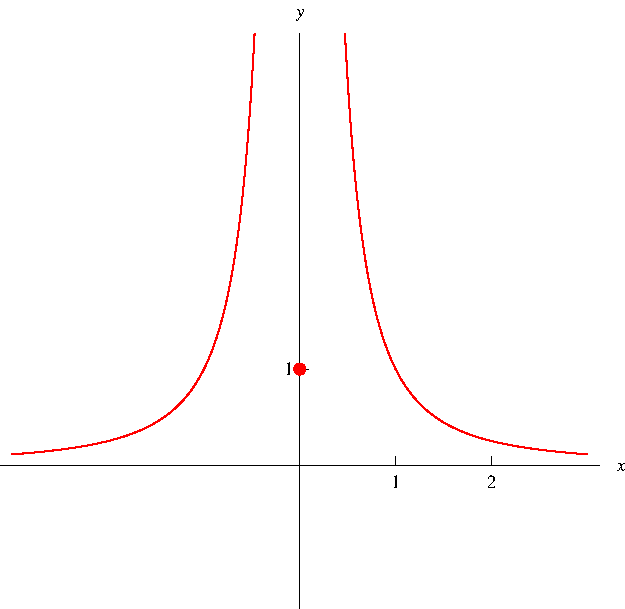
\includegraphics[height=4.5cm]{continuity/pictures/02-05-ex2b.pdf}%
\column{.6\textwidth}
\begin{itemize}
\item<2-| alert@3-4>  $f(0)$ \uncover<4->{is defined ($f(0) = 1$).}
\item<2-| alert@5-6>  $\lim\limits_{x\rightarrow 0} f(x)$ \uncover<6->{doesn't exist ($\infty$).}
\item<7->  Discontinuous at 0.
\item<8->  This is called an infinite discontinuity because the limit of the function is infinite.
\end{itemize}
\begin{definition}<9->
In general, $ f $ has an \textbf{infinite discontinuity} at $ x=a $ if $ \ds \lim_{x\to a^-}f(x)=\pm \infty $ or $ \ds \lim_{x\to a^+}f(x)=\pm \infty $.
\end{definition}
\end{columns}
\end{example}
\end{frame}


\begin{frame}
\begin{example} %[Example 2c, p. 114]
Where is this function discontinuous?
\begin{columns}[c]
\column{.4\textwidth}
\[
f(x) = \left\{ \begin{array}{lcl}
\frac{x^2 - x - 2}{x-2} & \text{ if } & x \neq 2 \\
\alert<handout:0 |4>{1} & \alert<handout:0 |4>{\text{ if }} & \alert<handout:0 |4>{x = 2} \\
\end{array}\right.
\]
\psset{xunit=0.8cm, yunit=0.8cm}
\begin{pspicture}(-3, -2)(3,4)
\psframe*[linecolor=white](-3,-2)(3,4) \psaxes[labels=none]{<->}(0,0)(-3,-2)(3,4)
\psplot[linecolor=red, plotpoints=1000]{-3}{3}{x 1 add }
\fcHollowDot{2}{3}
\fcFullDot{2}{1}
\end{pspicture} %
%\ 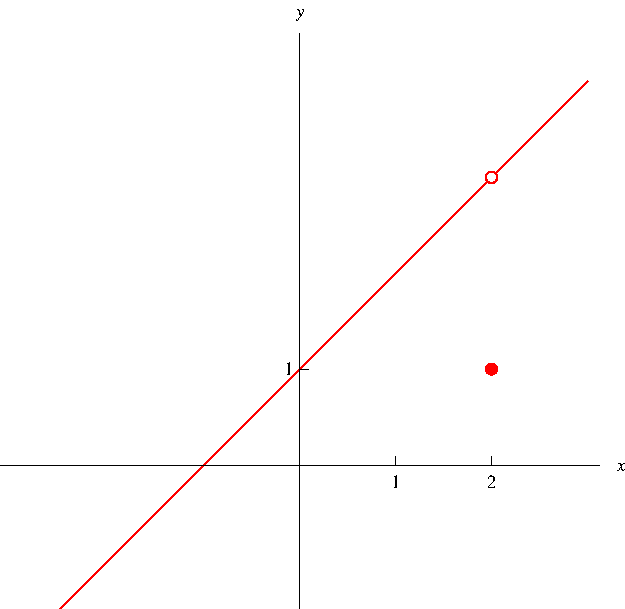
\includegraphics[height=4.5cm]{continuity/pictures/02-05-ex2c.pdf}%
\column{.6\textwidth}
\begin{itemize}
\item<2-| alert@3-4>  $f(2)$ \uncover<4->{is defined ($f(2) = 1$).}
\item<2-| alert@5-6>  $\lim\limits_{x\rightarrow 2} f(x)$ \uncover<6->{exists ($=3$).}
\item<7->  $\lim\limits_{x\rightarrow 2}f(x) \neq f(2)$.
\item<8->  Discontinuous at 2.
\item<9->  This is a removable discontinuity.
\end{itemize}
\end{columns}
\end{example}
\end{frame}


\begin{frame} \frametitle{Jump Discontinuity}
\begin{example}[Greatest Integer Function, or Floor Function] 
%[Example 2d, p. 114]
Where is this function discontinuous?
\begin{columns}[c]
\column{.4\textwidth}
\[
f(x) = \lfloor x\rfloor
\]
\ \psset{xunit=1cm, yunit=1cm}
\begin{pspicture}(-1.5, -1.5)(3.8,3.8)
\psframe*[linecolor=white](-1.5,-1.5)(3.8,3.8)
\psaxes[labels=x, ticks=x]{<->}(0,0)(-1.5,-1.5)(3.8,3.8)
\psline(-0.1,1)(0.1,1)
\rput[b](-0.25, 1){$1$}
\psline[linecolor=red](-1,-1)(0,-1)
\fcFullDot{-1}{-1}
\fcHollowDot{0}{-1}

\psline[linecolor=red](0,0)(1,0)
\fcFullDot{0}{0}
\fcHollowDot{1}{0}

\psline[linecolor=red](1,1)(2,1)
\fcFullDot{1}{1}
\fcHollowDot{2}{1}

\psline[linecolor=red](2,2)(3,2)
\fcFullDot{2}{2}
\fcHollowDot{3}{2}

\psline[linecolor=red](3,3)(3.8,3)
\fcFullDot{3}{3}
%\fcHollowDot{4}{3}
\end{pspicture}
%\ 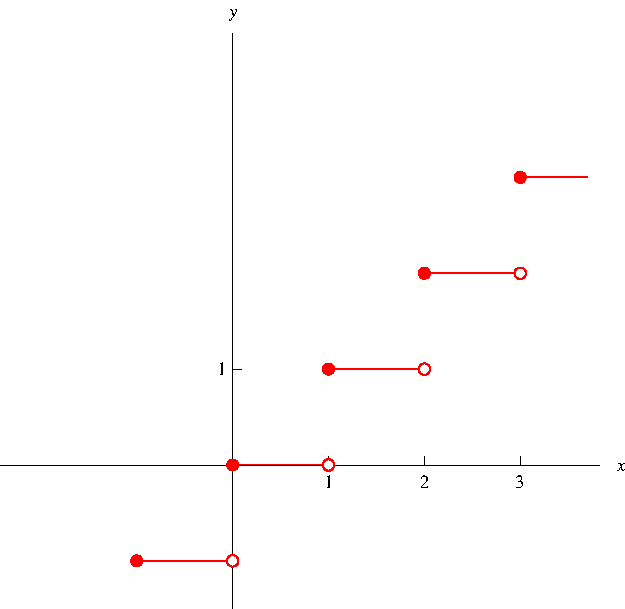
\includegraphics[height=4.5cm]{continuity/pictures/02-05-ex2d.pdf}%
\column{.6\textwidth}
\begin{itemize}
\item<2-| alert@3-4>  $f(1)$ \uncover<4->{exists ($f(1) = 1$).}
\item<2-| alert@5-6>  $\lim\limits_{x\rightarrow 1^+} f(x)$ \uncover<6->{$ = 1$.}
\item<2-| alert@7-8>  $\lim\limits_{x\rightarrow 1^-} f(x)$ \uncover<8->{$ = 0$.}
\item<2-| alert@9-10>  $\lim\limits_{x\rightarrow 1} f(x)$ \uncover<10->{doesn't exist.}
\item<11->  Discontinuous at 1.
\item<12->  Discontinuous at every integer $n$.
\item<13->  These are called \textbf{jump discontinuities} because the function ``jumps'' at these numbers (i.e., the left limit doesn't equal the right limit).
\end{itemize}
\end{columns}
\end{example}
\end{frame}
\begin{frame}
\begin{definition}
In general, $ f $ has a \textbf{jump discontinuity} at $ x=a $ if both $ \ds \lim_{x\to a^+} f(x) $ and $ \ds \lim_{x\to a^-} f(x) $ exist, but $ \ds \lim_{x\to a^+} f(x)  \ne  \lim_{x\to a^+} f(x) $.
\end{definition}

\vsp 

If the left and right limits disagree then of course it is impossible for the function value to agree with both.  However, it may be the case that the function value agrees with one of the on-sided limits  (as with the floor function). This motivates the following definition.   
\end{frame}
% end module continuity-ex2
